Para este projeto de controlador automático \emph{PID} será usado componentes eletrónicos discretos composto de amplificadores operacionais, sensores térmicos, bloco Peltier, resistores e capacitores os quais serão especificados no final da montagem de acordo como o \emph{as built}.\\
Porém, será agora especificado os componentes que serão usados na fase de projeto para obtenção dos parâmetros iniciais do projeto e que serão usados nas simulações no \emph{Simulink\tiny\textregistered} e \emph{Eletrical Work BanchSimulink\tiny\textregistered}.\\
\begin{enumerate}
\item \textbf{Bloco Peltier}\\
Este componente será usado com atuador de arrefecimento do sistema \emph{LASER} trazendo a temperatura para o \emph{set point} pré ajustado.\\
 Especificações do fabricante:
 
 %inicio das especificações do Peltier com imagem 
 
\begin{minipage}{0.5\linewidth}
%entrada da figura Peltier
\begin{figure}[H]
		\centering
		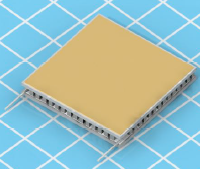
\includegraphics[width=0.4\linewidth]{./ima/peltiercatalogo01.png}
		\label{fig:Ppeltier02}
		\caption{Peltier - Catálogo}
	\end{figure}

\end{minipage} 

% Please add the following required packages to your document preamble:
% \usepackage[table,xcdraw]{xcolor}
% If you use beamer only pass "xcolor=table" option, i.e. \documentclass[xcolor=table]{beamer}
\begin{table}[H]
\centering
\caption{Catálogo Fabricante}
\label{datashittPeltier}
\begin{tabular}{|c|l|l|l|l|l|l|}
\hline
\rowcolor[HTML]{BBDAFF} 
\textbf{Type}                       & \multicolumn{1}{c|}{\cellcolor[HTML]{BBDAFF}\textbf{\begin{tabular}[c]{@{}c@{}}Dtmax\\ K\end{tabular}}} & \multicolumn{1}{c|}{\cellcolor[HTML]{BBDAFF}\textbf{\begin{tabular}[c]{@{}c@{}}Qmax\\ W\end{tabular}}} & \multicolumn{1}{c|}{\cellcolor[HTML]{BBDAFF}\textbf{\begin{tabular}[c]{@{}c@{}}Imax\\ A\end{tabular}}} & \multicolumn{1}{c|}{\cellcolor[HTML]{BBDAFF}\textbf{\begin{tabular}[c]{@{}c@{}}Umax\\ V\end{tabular}}} & \multicolumn{1}{c|}{\cellcolor[HTML]{BBDAFF}\textbf{\begin{tabular}[c]{@{}c@{}}AC R\\ ohm\end{tabular}}} & \multicolumn{1}{c|}{\cellcolor[HTML]{BBDAFF}\textbf{\begin{tabular}[c]{@{}c@{}}H\\ mm\end{tabular}}} \\ \hline
\multicolumn{7}{|c|}{1MX 06-063-xx ( N=126 núcleos )}                                                                                                                                                                                                                                                                                                                                                                                                                                                                                                                                                                                                                                       \\ \hline
\multicolumn{1}{|l|}{1MX 06-063-08} & 70                                                                                                      & 18.20                                                                                                  & 6.0                                                                                                    & 7.70                                                                                                   & 1.50                                                                                                      & 1.9                                                                                                  \\ \hline
\end{tabular}
\end{table}

\newpage

 
\end{enumerate}



